\chapter{Introduction}
This chapter is partially based on the authors PhD symposium paper~\cite{combiningLDandIR} and presents the overall motivation, structure and scientific contribution of this thesis.

\section{Motivation}
%Being a part of the \emph{Information Age}, users are challenged with a growing amount of Web data in unstructured, semi-structured and structured formats.
Since the proposal of hypertext from Tim-Berners Lee to his employer CERN at March 12, 1989\footnote{\url{http://www.w3.org/People/Berners-Lee/Longer.html}} the World Wide Web gathered more than one billion web pages and still grows exponentially\footnote{\url{http://www.internetlivestats.com/total-number-of-websites/}}.
Ten years later and with the advent of search engines, mankind became trained to find information by typing keywords and to expect several web documents in return~\cite{ilprints361}.

The access to this data 


However, already the Baseball system~\cite{green1961baseball} by Green et al. identified natural language as the most effective and convenient way to communicate information needs in computer communication.

Lunar\cite{woods1973progress}


Hence, computationally answering complex natural language questions over multiple data sources is a challenging research task demanding a solution composed of natural language processing, information retrieval and knowledge extraction abilities. 
In the last couple of years, the way search is perceived by end users as well as industrial agents changed dramatically.
In analogy, future developments in everyday and business search engines need to unlock the power of the underlying semantics of the data.

Building a novel question answering (QA) system over heterogeneous knowledge sources requires various building blocks.
For instance, named entity extraction approaches over unstructured data such as blogs, news or RSS feeds to capture the semantic meaning of a particular document.
Unfortunately, existing building blocks lack comparable evaluation settings, performance or quality. 

In this work, we identify three main challenges -- \emph{respectively research gaps} -- and present solutions for building basic components as well as whole systems for semantic question answering.
\begin{enumerate}
\item 
Over the last decades, several billion Web pages have been made available on the Web. 
The ongoing transition from the current \emph{Document Web} of unstructured data to the \emph{Data Web} yet requires scalable and accurate approaches for the extraction of structured data in RDF (Resource Description Framework) from these websites.
We address this key step for bridging the \emph{Semantic Gap}, i.e., extracting RDF from text,  with several approaches.
Our knowledge base-agnostic framework AGDISTIS can efficiently detect the correct URIs for a given set of named entities.
Furthermore, we present CETUS, an approach for recognizing entity types to populate RDF knowledge bases. 
\todo[inline]{@Axel: CDCR raus schmeißen?}
%Finally, we address the problem of assigning a single URI to named entities which stand for the same real-object across documents but are not yet available in the reference knowledge base.
\item 
This need to bridge between Document Web and the structured data on the Data Web has led to the development of a considerable number of annotation tools.
However, these tools are currently still hard to compare since the published evaluation results are calculated on diverse datasets and evaluated based on different measures
The resulting \emph{Evaluation Gap} is tackled by GERBIL, an evaluation framework for semantic entity annotation. The rationale behind our framework is to provide developers, end users and researchers with easy-to-use interfaces that allow for the agile, fine-grained and uniform evaluation of annotation tools on multiple datasets.
\item 
Finally, the decentral architecture behind the Web has led to pieces of information being distributed across data sources with varying structure. 
The search functionality to be developed in this thesis is going to be \emph{hybrid}, i.e., simultaneously performing a search on full-texts and semantic knowledge bases.
Different entity search algorithms need to be developed based on the significantly different data structures and problems arising from them. 
To close the arising \emph{Information Gap}, we introduce HAWK, a novel entity search approach for Hybrid Question Answering based on combining structured and unstructured data sources.
Moreover, we summarize existing solutions for semantic QA systems and propose an innovative architecture for self-improving, -healing and -wiring complex QA systems.
\end{enumerate}

Using the Semantic Web is expected to drive innovation in data integration and analysis software within companies. 
Moreover, end users anticipate more sophisticated search engines that understand complex natural language input, see for example Siri or Google Now.
\todo[inline]{cite or reformulate?}
Combining the advantages of information retrieval methods, question answering algorithms and semantic technologies will drive more sophisticated insights user-based, complex information needs.
However, there is yet no question answering framework which is able to convert the scientific advances, different research fields as well as hybrid knowledge sources into an usable system.














\section{Thesis Structure}

%Central to this PhD work is to answer \emph{how a search engine can benefit from the Linked Data paradigm?}
%Diverse technologies like RDFa, micro-data and HTML5 semantic annotations have been introduced to enrich Web data for a better user experience and machine interoperability.
%However, to the best of our knowledge there is no information retrieval architecture that uses the advantages of this technology holistically. 
%Moreover, some search pipeline steps for the Web of Data need to be revised in order to perform efficient and effective searches.

%To meet this obstacle, the presented thesis introduces a pipeline architecture for a Linked Data-based search engine, as depicted in Figure~\ref{overview}.

%\begin{figure*}[h!tb]
%    \centering
%        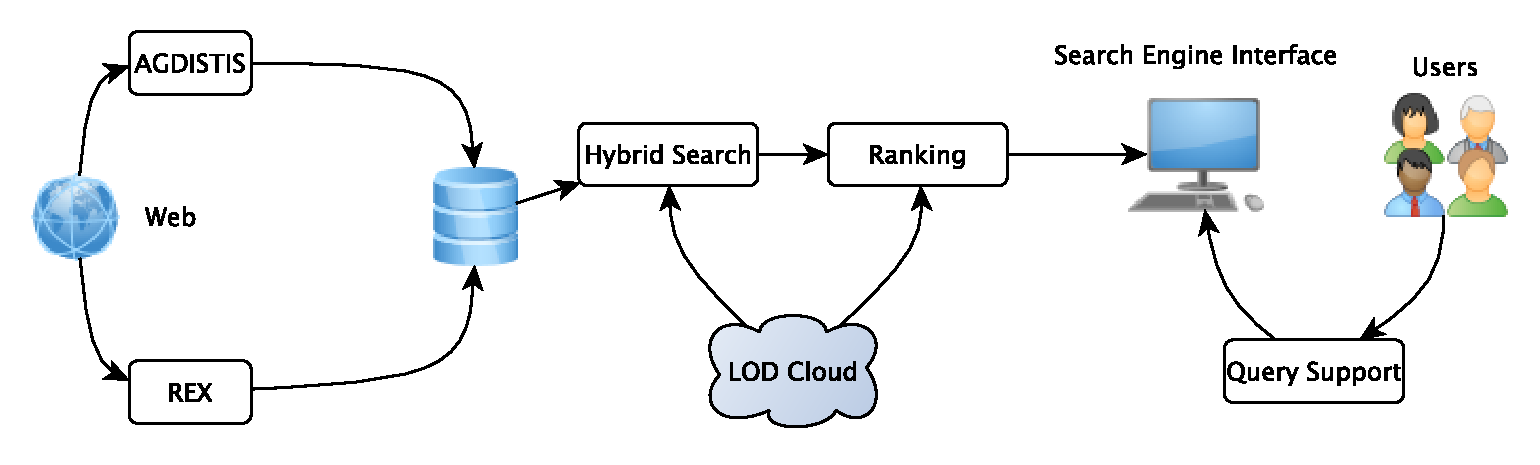
\includegraphics[width=\linewidth]{part_01/overview.pdf}
%    \caption{Overview of the proposed information system architecture.}
%    \label{overview}
%\end{figure*}

%The starting point of the proposed architecture is a two-fold data acquisition strategy based on a highly efficient, state-of-the-art industry Web crawler provided by our research partner \emph{Unister GmbH}.  

First, \emph{unstructured Web pages} from the crawled dataset, e.g., provided texts from news portals or agencies, are annotated by a standard NER algorithm~\cite{stanford} followed by a novel NED approach AGDISTIS~\cite{AGDISTIS}.
This NED approach has been developed to support arbitrary Linked Data knowledge bases to ensure future developments.
Moreover, AGDISTIS uses several NLP techniques to identify a set of candidate entities and identifies the correct with the help of the graph-based HITS algorithm. % and the resulting authority scores.
To prove the quality of AGDISTIS' results several corpora have been generated, evaluated and published. 
These corpora, called $N^3$~\cite{n3}, use the state-of-the-art serialization format \emph{NIF}~\cite{NIF} following the ``eating our own dogfood'' paradigm inherent to the Semantic Web community. 
$N^3$ are expected to form a novel gold standard in the areas of semantic named entity recognition and disambiguation.
Using $N^3$ and other well-known datasets, AGDISTIS has been proven to outperform the state-of-the-art algorithm AIDA~\cite{AIDA} by up to $16\%$ F-measure.
In the future, AGDISTIS will be evaluated against the framework of Cornolti et al.~\cite{cornolti} to provide a more comprehensive evaluation. 

Second, \emph{templated Web pages}, e.g., \url{http://www.imdb.com}, have been identified as another important source for answering user searches.
Therefore, REX~\cite{REX} has been developed during the early stage of this PhD work.
It is a web-scale semantic relation extraction framework capable to identify known as well as novel relations on Web pages creating RDF out of them.
REX combines a well-known wrapper induction technique~\cite{Crescenzi2013} for extracting XPath expressions, AGDISTIS as its NED algorithm and a consistency checker for the extracted relations based on ad-hoc generated schemas.
It has been shown that REX is able to generate new Linked Data triples with a precision of above $75\%$~\cite{REX}.

The resulting data from both pre-processing steps will serve as the underlying dataset for future research steps together with knowledge from the LOD Cloud.

Concerning the users' need for exploring the data space, %by enabling searches via keywords, natural language or even questions 
the next step is to \emph{support the formulation of queries}.
A huge potential within classical search engines is contained in inexact search queries, e.g., in terms of given a description only or a question.
Standard search engine methodologies fail at this point due to not being able to match keyword queries. 
In this thesis, we will support query formulation by providing on-the-fly recommended queries based on the real-time user input.
It is planned to use Linked Data such as \emph{BabelNet}\footnote{\url{http://babelnet.org/}} to find polysemes and synonyms within a query and thus enhancing the understanding of what the users actually mean.
Furthermore, three different standard approaches as well as a Linked Data-based grammar will be compared and evaluated against each other.
Another by-product of an according auto-completion approach is to teach the user which queries a search engine understands.

The research field of information retrieval/search and ranking has so far only been analysed theoretically within this doctoral work. 
In this thesis, a hybrid search engine is going to be implemented, i.e., an engine comprising a full-text information retrieval system enhanced by extracted Linked Data and a stake of LOD Cloud-based entity search.
Especially, the keyword-based search engine \emph{SINA}~\cite{sina} will be a starting point for further research. 

With respect to ranking algorithms, this PhD work focuses on two different research plans.
At first, a semantic extension of graph-based authority calculating algorithms will be investigated. 
Therefore, a master thesis has been looked after which analysed a context-driven enhancement of Stoyanovich's work~\cite{Stoyanovich}.
Initial results show an improvement compared to the baseline using the plain PageRank algorithm.
In parallel, an ensemble learning approach of Semantic Web-based ranking algorithms will be evaluated.

To summarize, the aforementioned steps will help building an integrated information system leveraging search engine performance using Linked Data.
Additionally--due to strong industry needs--this framework is going to be used in a real-life environment with web-scale amounts of users.
Finally, most of the source code will be published as open source and can be downloaded via the projects homepage\footnote{\url{http://aksw.org/RicardoUsbeck}}.

\section{Scientific Contributions}
This PhD work is dimensioned for three years. 
After intense literature reviews in the beginning of the first year the need for annotated Web data has been identified.
As a logical consequence, the development of AGDISTIS and REX had been finished by the end of the first year. 
Alongside, a gold standard ($N^3$) has been created to be able to evaluate the approaches mentioned above.

The second year will be used for developing and assessing the corresponding search and ranking procedures. 
To measure the quality of the \emph{auto-completion} technology, we assess different real-world query logs from our industry partner.
Thereby, we analyze how much characters are need to understand the query correct.
Additionally, we focus on the efficiency of the system in terms of milliseconds to react on a pressed key.

Considering the ranking evaluation, we will use standard precision, recall and f-measures as well as rank comparision measures, e.g., mean reciprocal rank. 
The underlying data is provided by the industry partner through human rater assessments and several comparisons to real-life search engines, e.g., Google or Wolfram Alpha.

Afterwards, the combined pipeline itself will be evaluated in a qualitative study using professionals and end users.
Therefore, empirical methods like Likert-scale questionnaires and direct relevance feedback will be used.


Next to refining already submitted work and optimizing the source code to meet industrial production standards, the developed approaches and algorithms will be refined in a spiral way if unpredictable results occur.
Thereby, upcoming ideas will be interweaved with the presented schedule creating a closed loop consisting of research question, development, evaluation and new research questions.